\documentclass[12pt,a4paper]{article}
\usepackage{amsmath}
\usepackage{amsfonts}
\usepackage{amssymb}
\usepackage{graphicx}
\usepackage{secdot}
\usepackage{multirow}
\usepackage[left=2cm,right=2cm,top=2cm,bottom=2cm]{geometry}

\title{{Experiment - 9\\ \textbf{ Lift and Drag measurement on symmetrical airfoil NACA0015 at different angles of attack}}}
\author{Arka Pramanick, AE21B007\\ Department of Aerospace Engineering\\ IIT Madras\\[3ex] Instructor:\\ \large Professor Dr. R. Sriram}

\date{17 April, 2023}


\begin{document}
\maketitle

\hline

\section{Aim :}
\begin{itemize}
    \item To measure value of Lift and Drag.
    \item To compare Lift Coefficients and Drag Coefficients with different Angles of Attack and Airspeed(or Reynolds No.)
\end{itemize}


\section{Apparatus :}
Required apparatus for performing this experiment are:
\begin{itemize}
    \item Manometer
    \item C15-10 Armfield tunnel
    \item Pitot-static Probe
    \item Fan
    \item Symmetrical Airfoil model
\end{itemize}



\newpage
\section{Theory :}
\begin{description}
   \item[Thin Airfoil NACA0015] The NACA 0015 is the airfoil from the 4-digit series of NACA airfoils.The airfoil is symmetrical and 00 denotes it has no chamber. The 15 indicates that the airfoil 
has a 15$\%$ thickness to chord length ratio.The parameters of the airfoil are followings:
\begin{itemize}
    \item Chord length of the airfoil(C) = 65 mm = 0.065 m
    \item Span length(L) = 150 mm = 0.15 m
\end{itemize}
\end{description}
\underline{\textbf{Stagnation and Static Pressure:}}
$\bold{Stagnation \hspace{2 mm} pressure}(P_{stag})$ is the pressure at the stagnation points in the fluid flow.\\
\\$\bold{Static \hspace{2mm} pressure}(P_{\infty})$ is the actual thermodynamic pressure of a flow.
$$  P_{stag} = P_{\infty} + \frac{\rho v^2}{2} $$
\underline{\textbf{Reynolds Number :}}
The $\bold{Reynolds \hspace{2mm} Number}$ is the ratio of inertial forces to viscous forces within a fluid that is subjected to relative internal moment due to variation of velocities.
$$  R_e = \frac{\rho V_{\infty} L}{\mu} $$
\underline{\textbf{Lift Force(L):}} $\bold{Lift}$ is the force on the body in a direction normal to the flow direction. The lift will only be 
presented if the fluid incorporates a circulatory flow about the body. As the velocity above the body is increased, the static pressure is reduced and the velocity beneath is 
decreased gives an increase in static pressure.\\
$$L = \int_{-\infty}^{\infty} \rho v (V_{\infty}-v)\,dx $$
\vspace{5mm}
\underline{\textbf{Coefficients of Lift($C_l$):}} The $\bold{Lift \hspace{2 mm} Coefficients}$ contains the effects of object shape, air viscosity, and compressibility. Lift coefficients are calculated by :  
$$ C_l = \frac{L}{(\rho V_{\infty}^2 A)/2} $$
\underline{\textbf{Drag Force(D):}} The $\bold{Drag}$ on  a  body in  an  oncoming flow  is the force on  the  body in  a  direction parallel to the flow. For small angles of attack, the lift force is high and the drag force is low.
Drag is calculated by: \\
$$D = \int_{-\infty}^{\infty} \rho v (V_{\infty}-v)\,dy $$
\underline{\textbf{Coefficients of Drag: }}  $\bold{Drag \hspace{2mm} Coefficients}$ caused due to skin friction and Drag. The drag coefficient is calculated by :
$$ C_d = \frac{D}{(\rho V_{\infty}^2 A)/2} $$ \\
$\rho$ = Density of Air = 1.225 $Kg/m^3$ , $V_{\infty}$ = Velocity of Air, A = ($C\times L$) = Area of Airfoil

\begin{figure}[!ht]
	\begin{center}
		\framebox{
			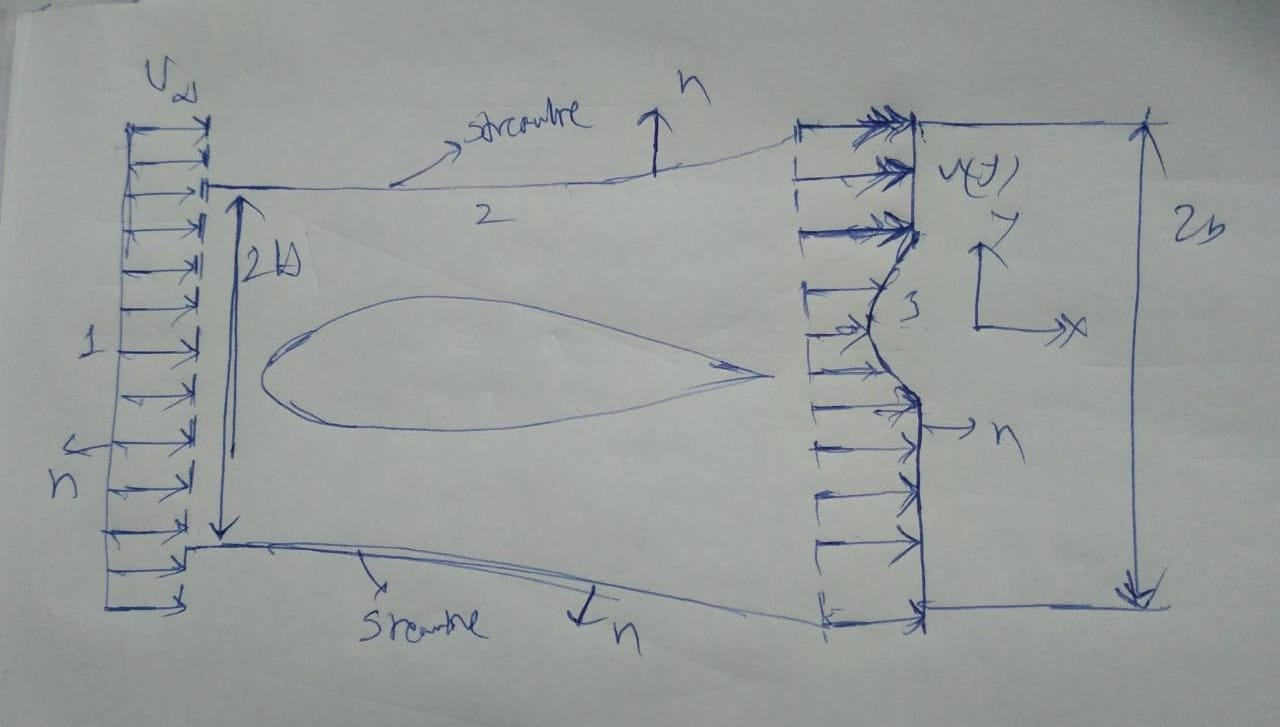
\includegraphics[scale=0.25]{8.1.jpg}
		}
	\end{center}
	\caption{Wake and Velocity profile behind a symmetric airfoil}
\end{figure}





\section{Procedure :}
\begin{enumerate}
    \item In wind tunnel test section is set.
    \item Pitot-static probe is connected to manometer.
    \item Fan speed is fixed.
    \item Required readings are taken.
\end{enumerate}






\section{Observation :}


\subsection{Required table for Drag Coefficients and Lift Coefficients :}
\begin{table}[ht]
\centering
\vspace{2mm}
\begin{tabular}{|p{15mm}|p{15mm}|p{15mm}|p{15mm}|p{15mm}|p{15mm}|p{15mm}|p{15mm}|p{15mm}|} 
 \hline
Angle of Attack($\alpha$) & \multicolumn{4}{|c|}{For velocity = 15 m/s} & \multicolumn{4}{|c|}{For Velocity = 20 m/s} \\ 
 \hline
  & Drag(D) & Lift(L) & $C_d$ & $C_l$ & Drag(D) & Lift(L) & $C_d$ & $C_l$ \\
 \hline
2 & 0.02 & 0.38  & 0.015 & 0.283 & 0.05 & 0.76 & 0.037 & 0.566\\ 
 \hline
 4 & 0.04 & 0.54 & 0.030 & 0.402 & 0.06 & 0.93 & 0.045 & 0.692 \\
 \hline
6 & 0.05 & 0.63 & 0.037 & 0.469 & 0.07 & 1.12 & 0.052 & 0.834  \\
 \hline
 8 & 0.07 & 0.75 & 0.052 & 0.558 & 0.09 & 1.36 & 0.067 & 1.012  \\
 \hline
10 & 0.12 & 0.8 & 0.089 & 0.595 & 0.12 & 1.56 & 0.089 & 1.161 \\
 \hline
12 & 0.18 & 0.75 & 0.134 & 0.558 & 0.17 & 1.58 & 0.134 & 1.176\\ 
 \hline
 \end{tabular}
\end{table}
\subsection{Plot of Lift Coefficients vs Angle of Attack}
\begin{figure}[!ht]
	\begin{center}
		\framebox{
			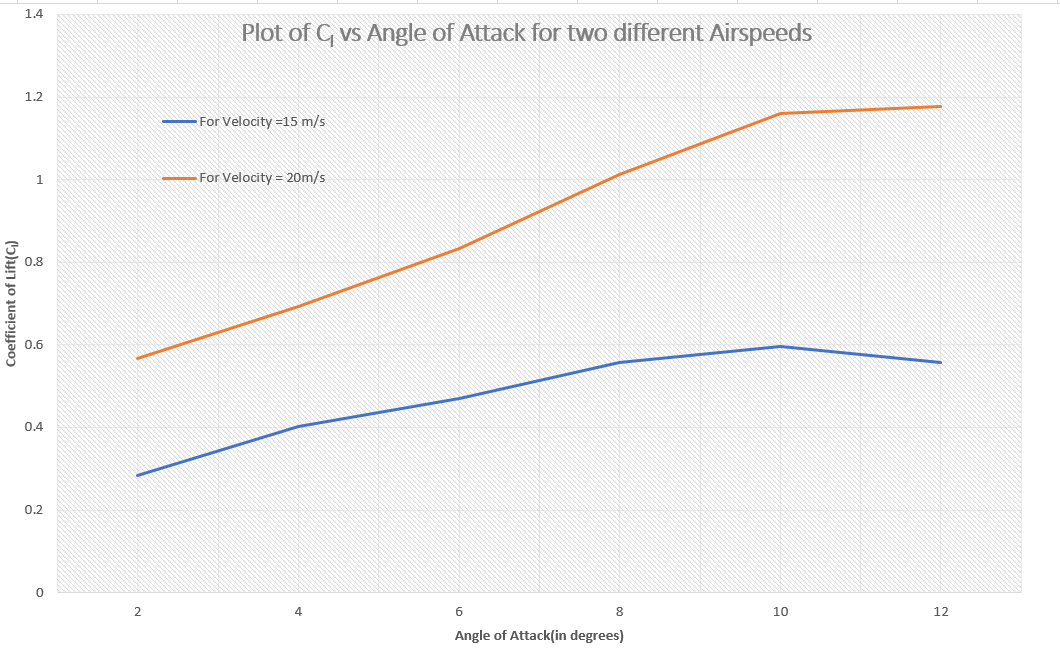
\includegraphics[scale=0.65]{expt 8.1.png}
		}
	\end{center}
	\caption{Plot of Coefficient of Lift VS Angle of Attack}
\end{figure}



\newpage









\newpage

\subsection{Plot of Coefficient of Lift vs Coefficient of Drag : } 



\begin{figure}[!ht]
	\begin{center}
		\framebox{
			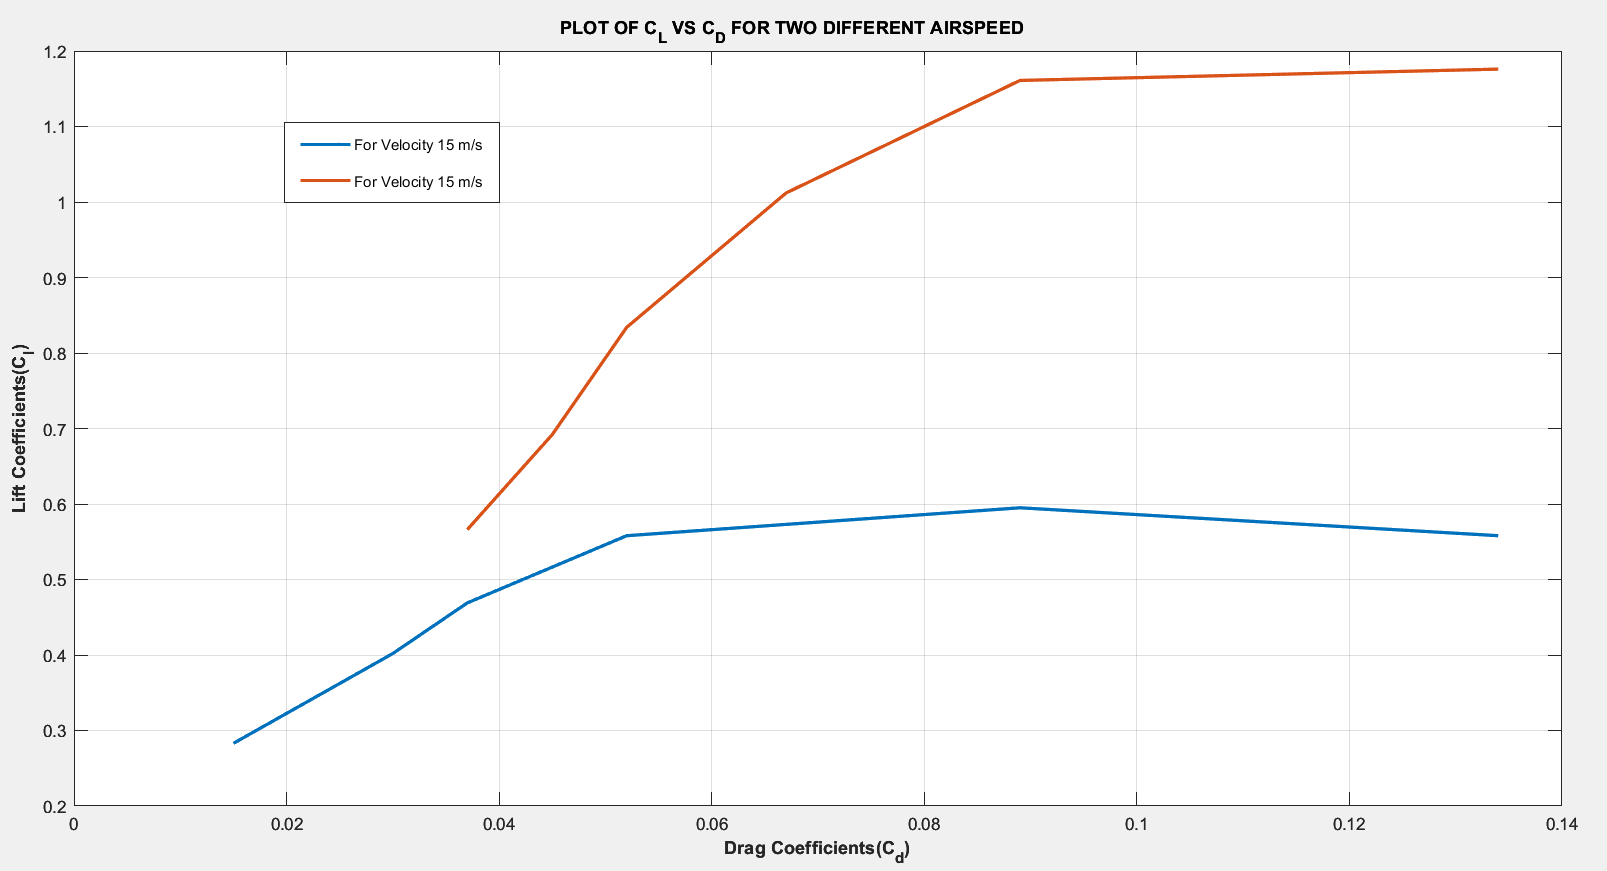
\includegraphics[scale=0.42]{9.2.png}
		}
	\end{center}
	\caption{Variation of Coefficients of Lift with Coefficient of Drag for Two different Velocities}
\end{figure}

\newpage


\section{Calculations :}
Density of air($\rho$) = 1.225 $\frac{Kg}{m^3}$ \\


\subsection{Calculation of Drag Coefficients :}
For Angle of Attack = 4 Degrees : \\
\underline{Velocity = 15 m/s} :\\
From experimental observation, \\
Drag(D) = 0.04 N\\
Area of Airfoil(A) = Chord Length(C)$\times$ Span Length(L) = 0.065$\times0.15 = 9.75 \times 10^{-3}$  \\
$$\Rightarrow C_d = \frac{2D}{\rho V_{\infty}^2 A}\\$$
$$\Rightarrow C_d = \frac{2\times 0.04}{1.225 \times 15^2 \times 9.75 \times 10^{-3}} $$
$$\Rightarrow \boxed{C_d = 0.030} $$


\subsection{Calculation of Lift Coefficients :}
For Angle of Attack = 4 Degrees : \\
\underline{Velocity = 15 m/s} :\\
From experimental observation, \\
Lift(L) = 0.54 N\\
Area of Airfoil(A) = Chord Length(C)$\times$ Span Length(L) = 0.065$\times0.15 = 9.75 \times 10^{-3}$  \\
$$\Rightarrow C_l = \frac{2L}{\rho V_{\infty}^2 A}\\$$
$$\Rightarrow C_l = \frac{2\times 0.04}{1.225 \times 15^2 \times 9.75 \times 10^{-3}} $$
$$\Rightarrow \boxed{C_l = 0.402} $$


\section{Sources of Error:}
\begin{itemize}
    \item Error due to instrumental defect.
    \item Error may occur in taking readings before flow becomes steady.
    \item Error due to environmental effect like temperature,pressure change.
    \item Error in measurement due to presence of zero error in parameters.
    \item Dimensional error may occurs .
    \item Parallax error may occur during set up of Angle of Attack.
\end{itemize}



\section{Conclusion :}
\begin{itemize}
    \item For small Angles of Attack Lift force is high and Drag Force is low.
    \item After a certain Angles of Attack  increases beyond a  
certain value, the lift force decreases and the drag forces increases.
    \item Both  lift and  drag coefficient  increases as  angle of attack  is 
increased. 
    \item After a certain Angle of attack($\bold{Stall Angle}$) Lift Coefficients decreases. For air speed = 15 m/s Stall Angle is 10 $^{\circ}$. Stall Angle is caused Due to transition of laminar to turbulence flow.
    \item Value of $C_l/C_d$ gradually decreases on increasing Angles of Attack.
    \item For each Angles of Attack $C_l$ is higher for flow with high Reynolds No.(or Airspeed).
\end{itemize}


\end{document}